% --+ SETUP +-------------------------------------------------------------------
\documentclass[aspectratio=169]{beamer}
\usepackage[utf8]{inputenc}
\usepackage[default]{lato}
% \usepackage[T1]{fontenc}
% \usepackage[ruled]{algorithm2e}
% \usepackage{amssymb}    % \lesssim and \gtrsim.
\usepackage{animate}
\usepackage{booktabs}   % Beautiful tabular.
\usepackage{empheq}
% \usepackage{hyperref}   % Hyperlinks.
% \usepackage{incgraph,tikz}
% \usepackage{incgraph}   % Include pdf file as page.
% \usepackage{multicol}
% \usepackage{pifont}
\usepackage{tabularx}   % \textwidth tabular.
% \usepackage{textgreek}  % Greek letters in text mode.

% --+ THEME +-------------------------------------------------------------------
% !TEX root = main.tex
\setbeamertemplate{navigation symbols}{}

% Custom commands.
\newcommand{\lsim}{\lesssim}
\newcommand{\gsim}{\gtrsim}
\newcommand{\cmark}{\ding{51}}
\newcommand{\xmark}{\ding{55}}
\newcommand{\done}{\rlap{$\square$}{\raisebox{2pt}{\large\hspace{1pt}\cmark}}%
\hspace{-2.5pt}}

% Tight fboxes.
\setlength{\fboxsep}{0pt}

% Fancy empheq box.
\newlength\mytemplen
\newsavebox\mytempbox

\makeatletter
\newcommand\eqbox{
    \@ifnextchar[
        {\@eqbox}
        {\@eqbox[0pt]}
}

\def\@eqbox[#1]{
    \@ifnextchar[
        {\@@eqbox[#1]}
        {\@@eqbox[#1][0pt]}
}

\def\@@eqbox[#1][#2]#3{
    \sbox\mytempbox{#3}
    \mytemplen\ht\mytempbox
    \advance\mytemplen #1\relax
    \ht\mytempbox\mytemplen
    \mytemplen\dp\mytempbox
    \advance\mytemplen #2\relax
    \dp\mytempbox\mytemplen
    \colorbox{color_box}{\hspace{1em}\usebox{\mytempbox}\hspace{1em}}
}

\makeatother

% custom overline from, https://tex.stackexchange.com/questions/22100/the-bar-and-overline-commands.
\makeatletter
\newsavebox\myboxA
\newsavebox\myboxB
\newlength\mylenA

\newcommand*\xoverline[2][0.75]{%
    \sbox{\myboxA}{$\m@th#2$}%
    \setbox\myboxB\null% Phantom box
    \ht\myboxB=\ht\myboxA%
    \dp\myboxB=\dp\myboxA%
    \wd\myboxB=#1\wd\myboxA% Scale phantom
    \sbox\myboxB{$\m@th\overline{\copy\myboxB}$}% Overlined phantom
    \setlength\mylenA{\the\wd\myboxA}% calc width diff
    \addtolength\mylenA{-\the\wd\myboxB}%
    \ifdim\wd\myboxB<\wd\myboxA%
       \rlap{\hskip 0.5\mylenA\usebox\myboxB}{\usebox\myboxA}%
    \else
        \hskip -0.5\mylenA\rlap{\usebox\myboxA}{\hskip 0.5\mylenA\usebox\myboxB}%
    \fi}

% Title page.
\defbeamertemplate*{title page}{customized}[1][]
{
    \vspace*{90pt}
    {\centering
        \usebeamerfont{title}\usebeamercolor[color_ef]{title}\textbf{\inserttitle}\par
        \usebeamerfont{author}\usebeamercolor[color_fg]{author}\insertauthor\par
    }
    \vskip72pt%
    {\centering
        \usebeamerfont{date}\insertdate\par
    }
    \vfill
}

% Add a number to each frame (but not the total number of frames!)
\addtobeamertemplate{navigation symbols}{}{
    \usebeamerfont{footline}
    \usebeamercolor[fg]{footline}
    \hspace{1em}
    \insertframenumber
}

% === EVERFOREST DARK HARD =====================================================
\definecolor{efd_bg}    {HTML}{272e33}
\definecolor{efd_fg}    {HTML}{d3c6aa}
\definecolor{efd_red}   {HTML}{e67e80}
\definecolor{efd_orange}{HTML}{e69875}
\definecolor{efd_yellow}{HTML}{dbbc7f}
\definecolor{efd_green} {HTML}{a7c080}
\definecolor{efd_dgreen}{HTML}{425047}
\definecolor{efd_aqua}  {HTML}{83c092}
\definecolor{efd_blue}  {HTML}{7fbbb3}
\definecolor{efd_purple}{HTML}{d699b6}

% === EMPHASIS COMMANDS ========================================================
\newcommand{\ef}[1]{\textbf{\textcolor{color_ef}{#1}}}
\newcommand{\eft}[1]{\texttt{\ef{#1}}}
\newcommand{\ered}   [1]{\textbf{\textcolor{efd_red}   {#1}}}
\newcommand{\eorange}[1]{\textbf{\textcolor{efd_orange}{#1}}}
\newcommand{\eyellow}[1]{\textbf{\textcolor{efd_yellow}{#1}}}
\newcommand{\egreen} [1]{\textbf{\textcolor{efd_green} {#1}}}
\newcommand{\eaqua}  [1]{\textbf{\textcolor{efd_aqua}  {#1}}}
\newcommand{\eblue}  [1]{\textbf{\textcolor{efd_blue}  {#1}}}
\newcommand{\epurple}[1]{\textbf{\textcolor{efd_purple}{#1}}}

% === APPENDIX REFERENCE =======================================================
\newcommand{\appref}[1]{\textsuperscript{\textcolor{efd_purple}{\ref{#1}}}}
\newcommand{\backref}[1]{
    \vskip0pt plus 1 filll
    \begin{flushright}
        \tiny{\textit{Ref'd by \textcolor{efd_purple}{\ref{#1}}.}}
    \end{flushright}
    \smallskip
}

% === THEME ====================================================================
% These three colors will be the palette of the presentation.
\colorlet{color_bg}{efd_bg}      % Background color of each slide.
\colorlet{color_fg}{efd_fg}      % Foreground color, mainly used by text.
\colorlet{color_ef}{efd_green}   % Emphasis color, uses for titles, etc.
\colorlet{color_box}{efd_dgreen} % Box color.

% Don't touch stuff beyond this point!
\setbeamercolor{normal text}{bg=color_fg,fg=color_fg}
\setbeamercolor{item}{bg=color_ef,fg=color_ef}
\setbeamercolor{background canvas}{bg=color_bg}
\setbeamercolor{palette primary}{bg=color_ef,fg=color_bg}
\setbeamercolor{palette secondary}{bg=color_fg,fg=color_bg}
\setbeamercolor{palette tertiary}{bg=color_fg,fg=color_bg}
\setbeamercolor{palette quaternary}{bg=color_fg,fg=color_bg}
\setbeamercolor{structure}{fg=color_ef} % itemize, enumerate, etc
\setbeamercolor{section in toc}{fg=color_ef} % TOC sections


% --+ TITLEPAGE SETUP +---------------------------------------------------------
\title{Acceptance Study of the CLAS12 Detector Using the Forward Micromegas Tracker for Run Group E}
\author{Bruno Benkel}
\date{2023-09-14}
% TODO. Add shit

% --+ DOCUMENT +----------------------------------------------------------------
\begin{document}
    \colorlet{color_ef}{efd_green}

    % --+ FIRST PAGES +---------------------------------------------------------
    % ------+ TITLEPAGE +-------------------------------------------------------
    \titlepage
    % ------+ SUMMARY & TABLE OF CONTENTS +-------------------------------------

    % --+ CONTEXT +-------------------------------------------------------------
    \graphicspath{{10context/img}}
    % !TEX root = main.tex
\begin{frame}{}
    \centering \Huge{\ef{Context}}
\end{frame}

% --+ PHYSICS +-----------------------------------------------------------------
% --+ CLAS12 +------------------------------------------------------------------
% --+ DOUBLE TARGET +-----------------------------------------------------------


    % --+ DATA ANALYSIS +-------------------------------------------------------
    \graphicspath{{11data_analysis/img}}
    % !TEX root = main.tex
\begin{frame}{}
    \centering \Huge{\ef{Context}}
\end{frame}

% --+ PHYSICS +-----------------------------------------------------------------
% --+ CLAS12 +------------------------------------------------------------------
% --+ DOUBLE TARGET +-----------------------------------------------------------


    % --+ STUDY RESULTS +-------------------------------------------------------
    \graphicspath{{12study_results/img}}
    % !TEX root = main.tex
\begin{frame}{}
    \centering \Huge{\ef{Context}}
\end{frame}

% --+ PHYSICS +-----------------------------------------------------------------
% --+ CLAS12 +------------------------------------------------------------------
% --+ DOUBLE TARGET +-----------------------------------------------------------


    % --+ APPENDICES +----------------------------------------------------------
    \colorlet{color_ef}{efd_purple}
    \graphicspath{{20appendices/img}}
    % !TEX root = ../main.tex
\section*{Appendices}
\addcontentsline{toc}{section}{Appendices}
\label{20::appendices}
    \renewcommand{\thesubsection}{\Alph{subsection}}
    % !TEX root = ../main.tex
\subsection{Reproducibility}
\label{20.01::reproducibility}
    In order to ensure the reproducibility of the research presented in this thesis, we provide access to all datasets and code used in the development of our study.
    We believe that transparency and accessibility are crucial for scientific integrity and to facilitate further investigations by the research community.

    We encourage interested readers and fellow researchers to access and utilise these resources for the purpose of reproducibility and advancing scientific knowledge.
    Should there be any inquiries or issues regarding the datasets or code, please do not hesitate to contact the author at \href{mailto:bruno.benkel@gmail.com}{\texttt{bruno.benkel@gmail.com}} for further assistance.

    We believe that open access to data and code fosters collaboration, accelerates scientific progress, and ensures the robustness of research findings.
    By making these resources available, we aim to contribute to the collective effort of reproducible and transparent scientific research.

    % --+ Datasets +------------------------------------------------------------
    \paragraph{Datasets}
        Regrettably, there is no website or location to openly share datasets in the \textit{Universidad Técnica Federico Santa María} (UTFSM) or the \textit{Centro Científico Tecnológico de Valparaíso} (CCTVal).
        For readers with access to the JLab farm, all used datasets are available at

        \begin{center}
            \texttt{/work/clas12/users/benkel/thesis-datasets}
        \end{center}

        For individuals who do not have access to the JLab farm, please feel free to contact the author, and we will explore alternative methods to share the relevant datasets.

    % --+ Code +----------------------------------------------------------------
    \paragraph{Code}
        The sources for the code used for data processing, analysis, and generating figures are shared on Table \ref{tab::20.01::code_locations}.
        By providing the code, we aim to enable researchers to replicate our findings, perform additional analyses, or build upon our work.

        \begin{table}[b!]
            \begin{center}
                \begin{tabularx}{0.90\textwidth}{ll}
                    \toprule
                    \textbf{Software}  & \textbf{Link} \\
                    \midrule \midrule
                    RG-E Slow Controls &
                        \href{https://github.com/bleaktwig/rge-epics-support}
                        {\texttt{github.com/bleaktwig/rge-epics-support}} \\
                    \midrule
                    CLAS12 Alignment   &
                        \href{https://github.com/JeffersonLab/clas12alignment}
                        {\texttt{github.com/JeffersonLab/clas12alignment}} \\
                    \midrule
                    thesis-simul       &
                        \href{https://github.com/bleaktwig/thesis-simul}
                        {\texttt{github.com/bleaktwig/thesis-simul}} \\
                    thesis-data        &
                        \href{https://github.com/bleaktwig/thesis-data}
                        {\texttt{github.com/bleaktwig/thesis-data}} \\
                    RG-E Analysis      &
                        \href{https://github.com/bleaktwig/clas12-rge-analysis}
                        {\texttt{github.com/bleaktwig/clas12-rge-analysis}} \\
                    GEMC               &
                        \href{https://github.com/gemc/source}
                        {\texttt{github.com/gemc/source}} \\
                    Coatjava           &
                        \href{https://github.com/JeffersonLab/coatjava}
                        {\texttt{github.com/JeffersonLab/coatjava}} \\
                \bottomrule
            \end{tabularx}
        \end{center}

        \caption{Table with code locations.}
        \label{tab::20.01::code_locations}
    \end{table}

    % !TEX root = ../main.tex
\addcontentsline{toc}{subsection}{RG-F Target Layout}
\label{20.02::rgf_target_layout}
    \incgraph[documentpaper,][width=\paperwidth,height=\paperheight]{20addenda/img/02rgf_target_layout.pdf}
    % TODO. Once done with addenda, change title of pdf to the correct addendum number.

    % !TEX root = ../main.tex
\subsection{FMT Layer Efficiency Error Estimation}
\label{20.03::fmt_layer_efficiency_error_estimation}
    This Appendix presents the Python script described in Section \ref{14.14::efficiency_study}.
    The script utilises the formulae outlined in that section to estimate the errors in the efficiency of the 2-layer and 3-layer tracks.
    It should be noted, as mentioned in the section, that the efficiency $E_{1(2)}$ (referred to as \verb|E12| in the code) was obtained through numerical methods.

    \begin{lstlisting}[language=Python]
    import sys
    def printf(format, *args):
        sys.stdout.write(format % args)
    def f_E13(E3):
        return E3**(1/3)
    def f_E1(E12, E13):
        return (4*E12 + E13)/5
    def f_dE12(E1, E12):
        return abs(E1 - E12)
    def f_dE13(E1, E13):
        return abs(E1 - E13)
    def f_dE2(E12, dE12):
        return (6*E12 - 9*E12**2) * dE12
    def f_dE3(E13, dE13):
        return 3*E13**2 * dE13

    # Input.
    #      Run 12933.                    Run 12016.
    E2  = [.251,.065,.056,.375,.137,.142,.327,.111,.089,.537,.280,.295]
    E3  = [.056,.003,.003,.085,.007,.007,.099,.010,.009,.164,.027,.029]
    E12 = [.306,.157,.144,.402,.239,.244,.339,.206,.180,.497,.364,.377]

    # Run functions.
    E13  = list(map(f_E13,  E3))
    E1   = list(map(f_E1,   E12, E13))
    dE12 = list(map(f_dE12, E1,  E12))
    dE13 = list(map(f_dE13, E1,  E13))
    dE2  = list(map(f_dE2,  E12, dE12))
    dE3  = list(map(f_dE3,  E13, dE13))

    # Print.
    print("dE2:")
    for i in dE2:
        printf("%5.1f,", 100*i)
    print("dE3:")
    for i in dE3:
        printf("%5.1f,", 100*i)
    \end{lstlisting}

    % !TEX root = ../main.tex
\subsection{DIS plots in $v_z$ bins}
\label{20.04::dis_vz_plots}
    In Section \ref{14.31::phase_space_study}, we presented the acceptance-corrected DIS variables separated into $v_z$ bins.
    In this Appendix, we provide the same distributions without applying the acceptance correction.
    The statistics are considerably lower in $v_z$ bins characterised by low acceptance, such as $v_z > 10$ cm.
    This effect is more pronounced for the hadronic variables, as one would expect.
    Moreover, the correction noticeably alters the shape of certain distributions, bringing them closer to the expected theoretical behaviour.
    A clear illustration of this can be observed in the disparity of $Q^2$ depicted in Figures \ref{fig::14.31::q2_vz} and \ref{fig::20.04::q2_vz}, as well as in the dissimilarity of $z_h$ demonstrated in Figures \ref{fig::14.31::zh_211_vz} and \ref{fig::20.04::zh_211_vz}.

    % Q2.
    \begin{figure}
        \centering
        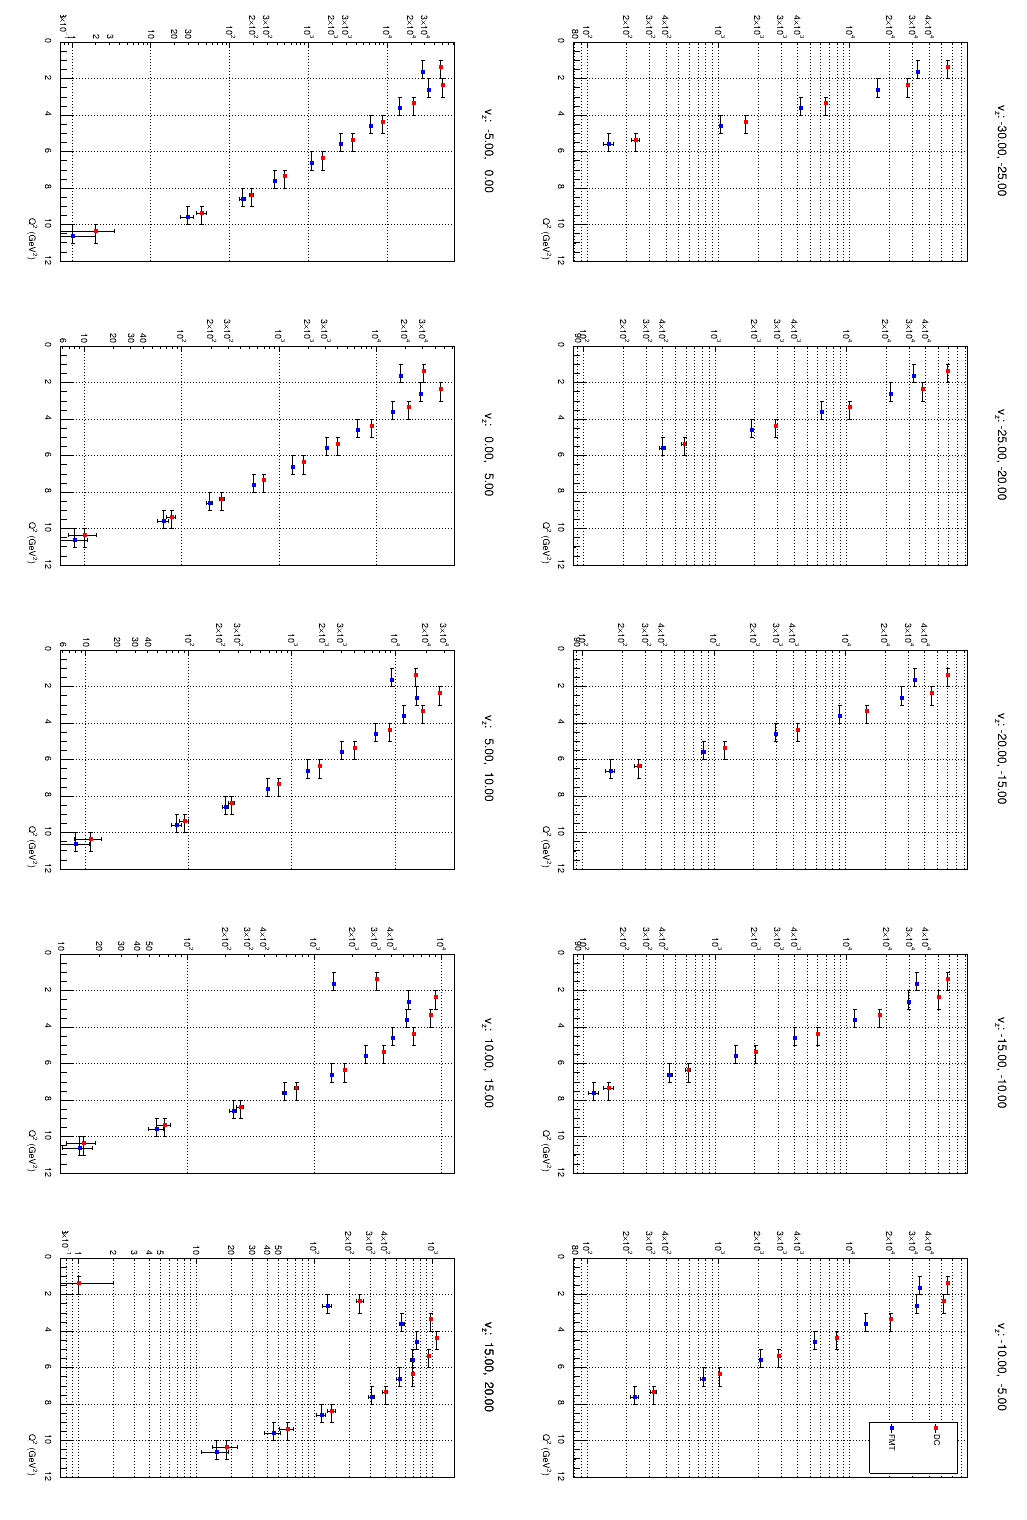
\includegraphics[width=\textwidth]{04q2_vz.png}
        \caption[$Q^2$ separated in $v_z$ bins]
        {$Q^2$ detected by DC and FMT, separated in $v_z$ bins.
        Run 12016.
        The bin markers are slightly shifted in $x$ to improve legibility.}
        \floatfoot{Source: Own elaboration, using the \href{https://github.com/bleaktwig/clas12-rge-analysis}{clas12-rge-analysis} software.}
        \label{fig::20.04::q2_vz}
    \end{figure}

    % nu.
    \begin{figure}
        \centering
        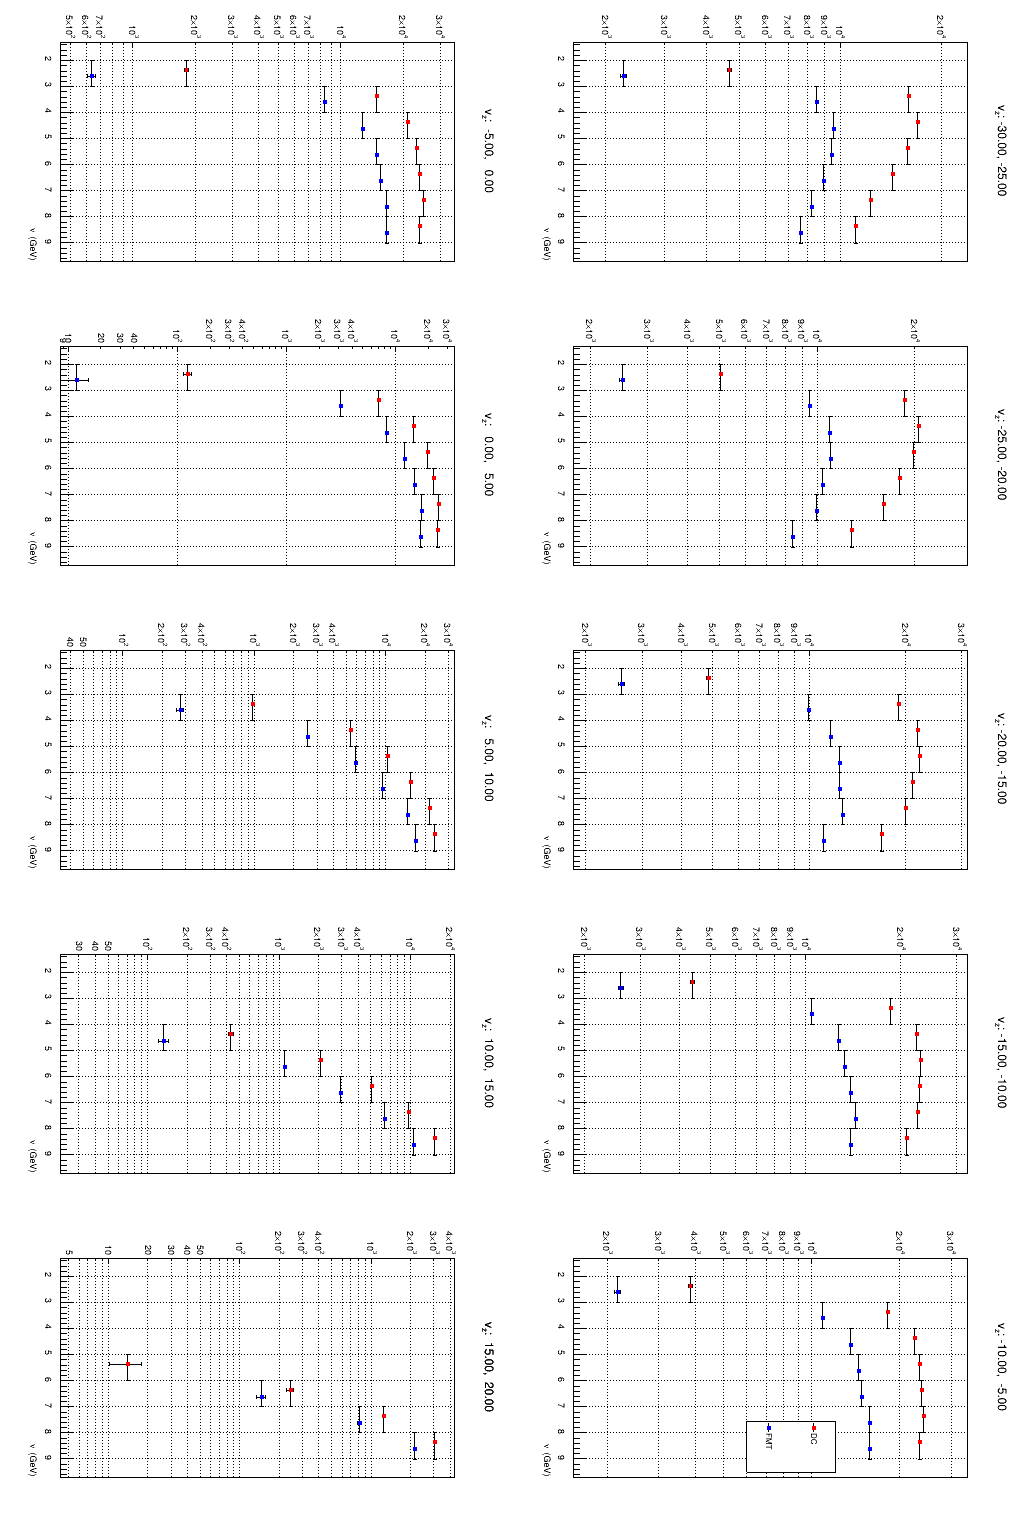
\includegraphics[width=\textwidth]{04nu_vz.png}
        \caption[$\nu$ separated in $v_z$ bins]
        {$\nu$ detected by DC and FMT, separated in $v_z$ bins.
        Run 12016.
        The bin markers are slightly shifted in $x$ to improve legibility.}
        \floatfoot{Source: Own elaboration, using the \href{https://github.com/bleaktwig/clas12-rge-analysis}{clas12-rge-analysis} software.}
        \label{fig::20.04::nu_vz}
    \end{figure}

    % zh.
    \begin{figure}
        \centering
        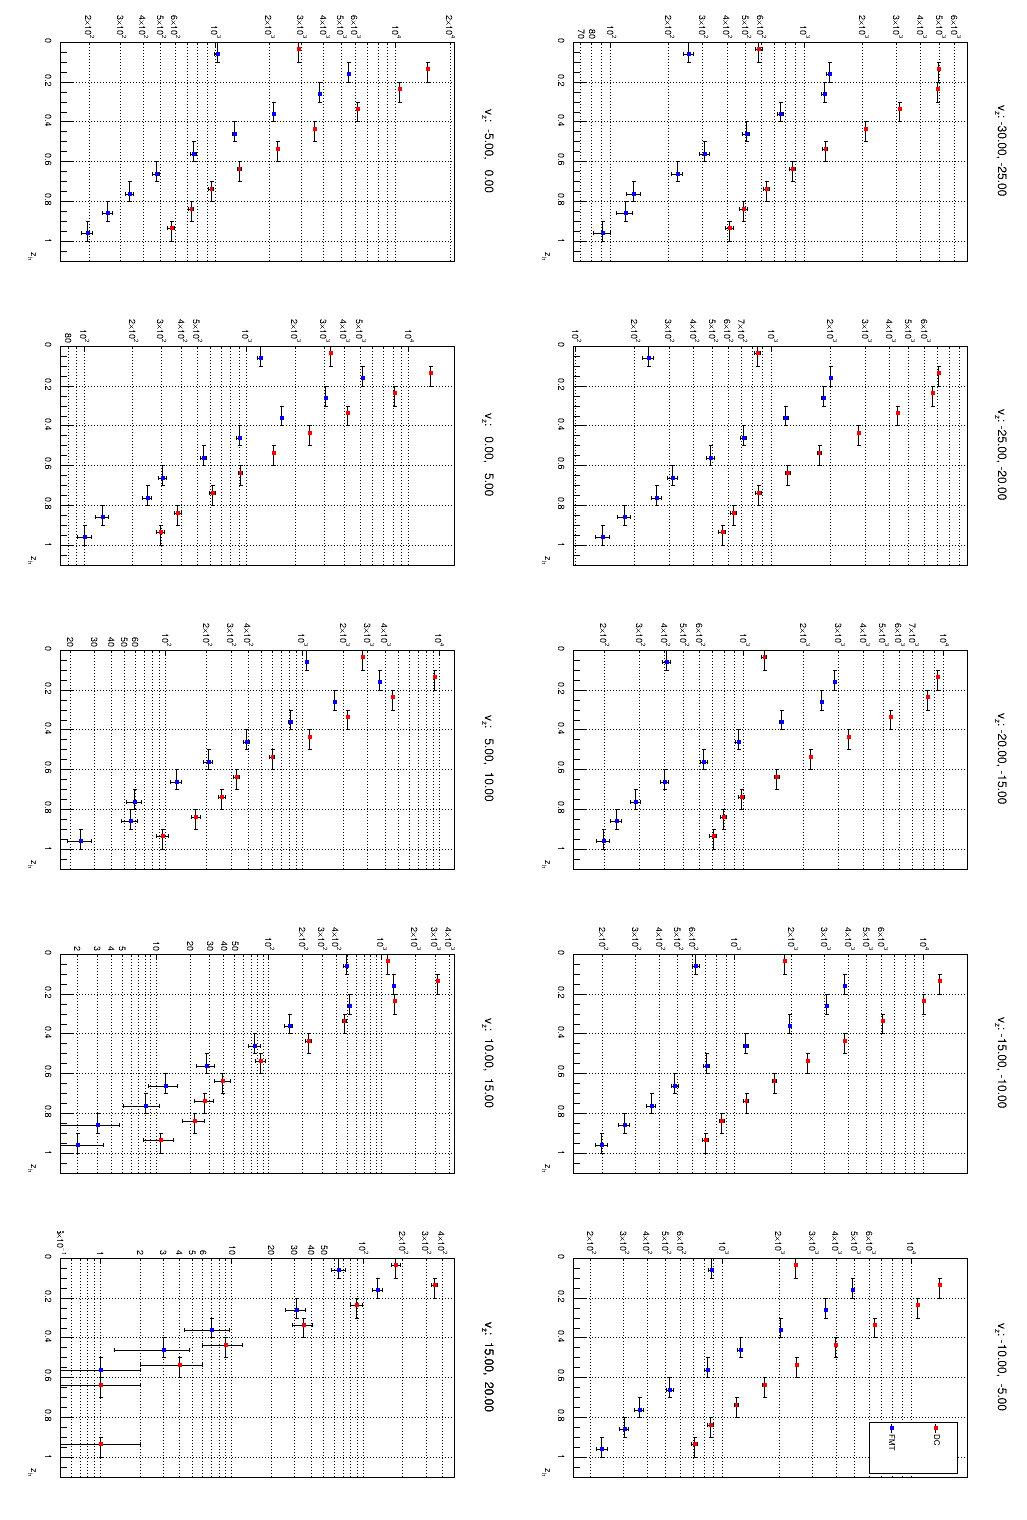
\includegraphics[width=\textwidth]{04zh_vz_211.png}
        \caption[$z_h$ for $e^-\pi^+$ separated in $v_z$ bins]
        {$z_h$ for $e^-\pi^+$ detected by DC and FMT, separated in $v_z$ bins.
        Run 12016.
        The bin markers are slightly shifted in $x$ to improve legibility.}
        \floatfoot{Source: Own elaboration, using the \href{https://github.com/bleaktwig/clas12-rge-analysis}{clas12-rge-analysis} software.}
        \label{fig::20.04::zh_211_vz}
    \end{figure}

    \begin{figure}
        \centering
        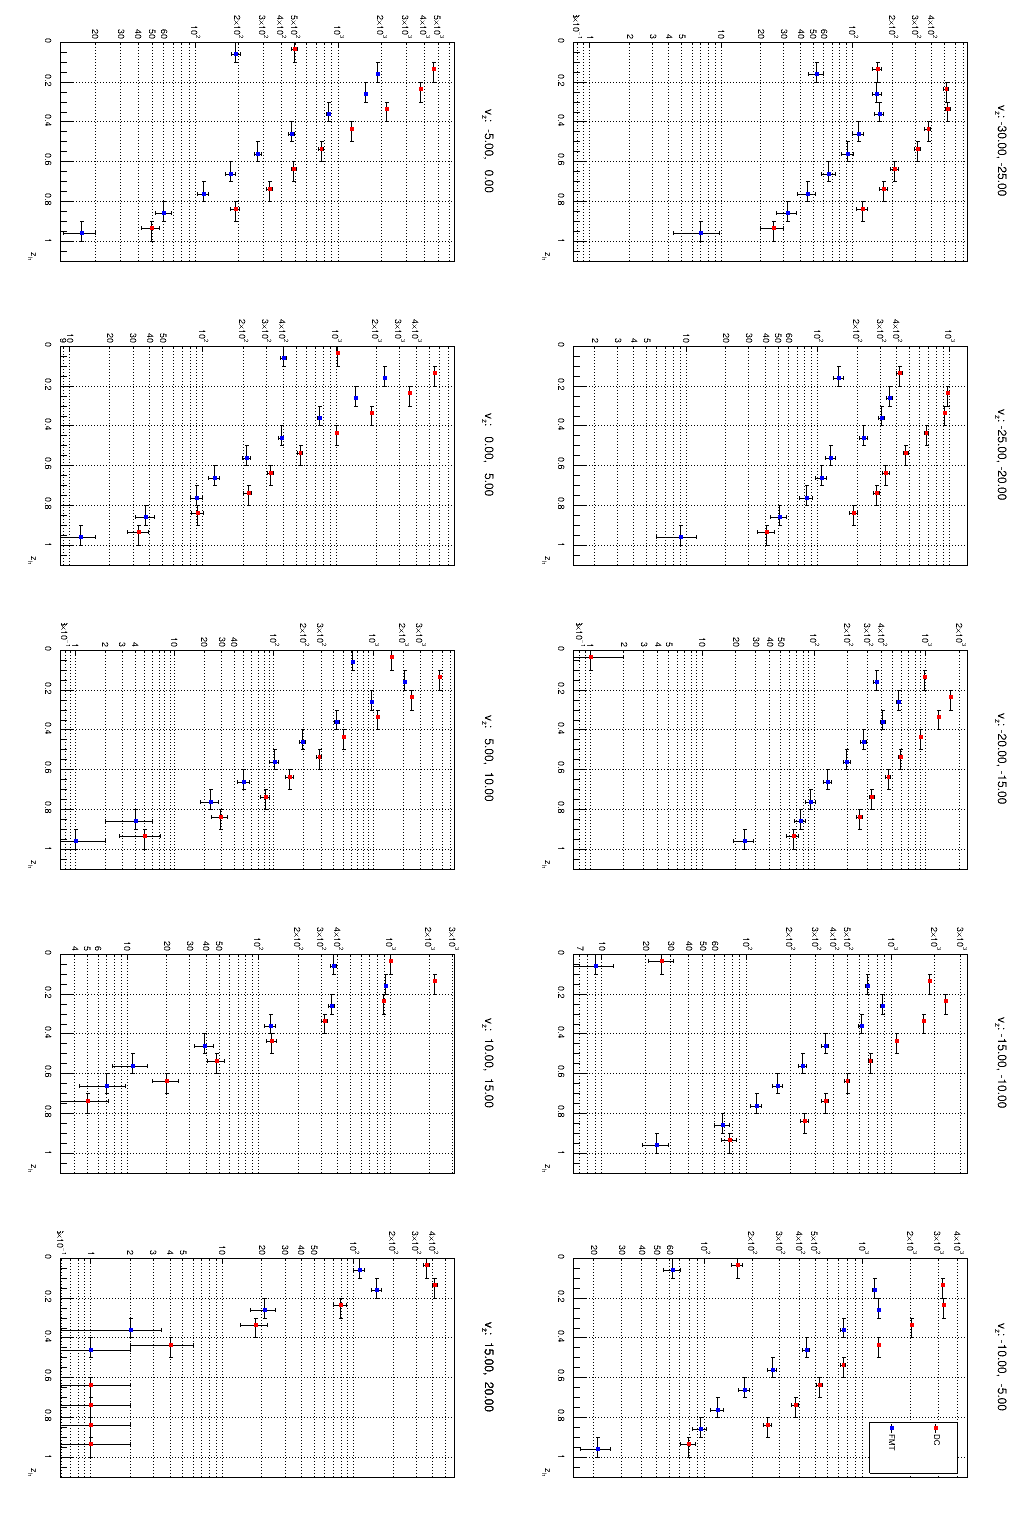
\includegraphics[width=\textwidth]{04zh_vz_-211.png}
        \caption[$z_h$ for $e^-\pi^-$ separated in $v_z$ bins]
        {$z_h$ for $e^-\pi^-$ detected by DC and FMT, separated in $v_z$ bins.
        Run 12016.
        The bin markers are slightly shifted in $x$ to improve legibility.}
        \floatfoot{Source: Own elaboration, using the \href{https://github.com/bleaktwig/clas12-rge-analysis}{clas12-rge-analysis} software.}
        \label{fig::20.04::zh_-211_vz}
    \end{figure}

    % pt2.
    \begin{figure}
        \centering
        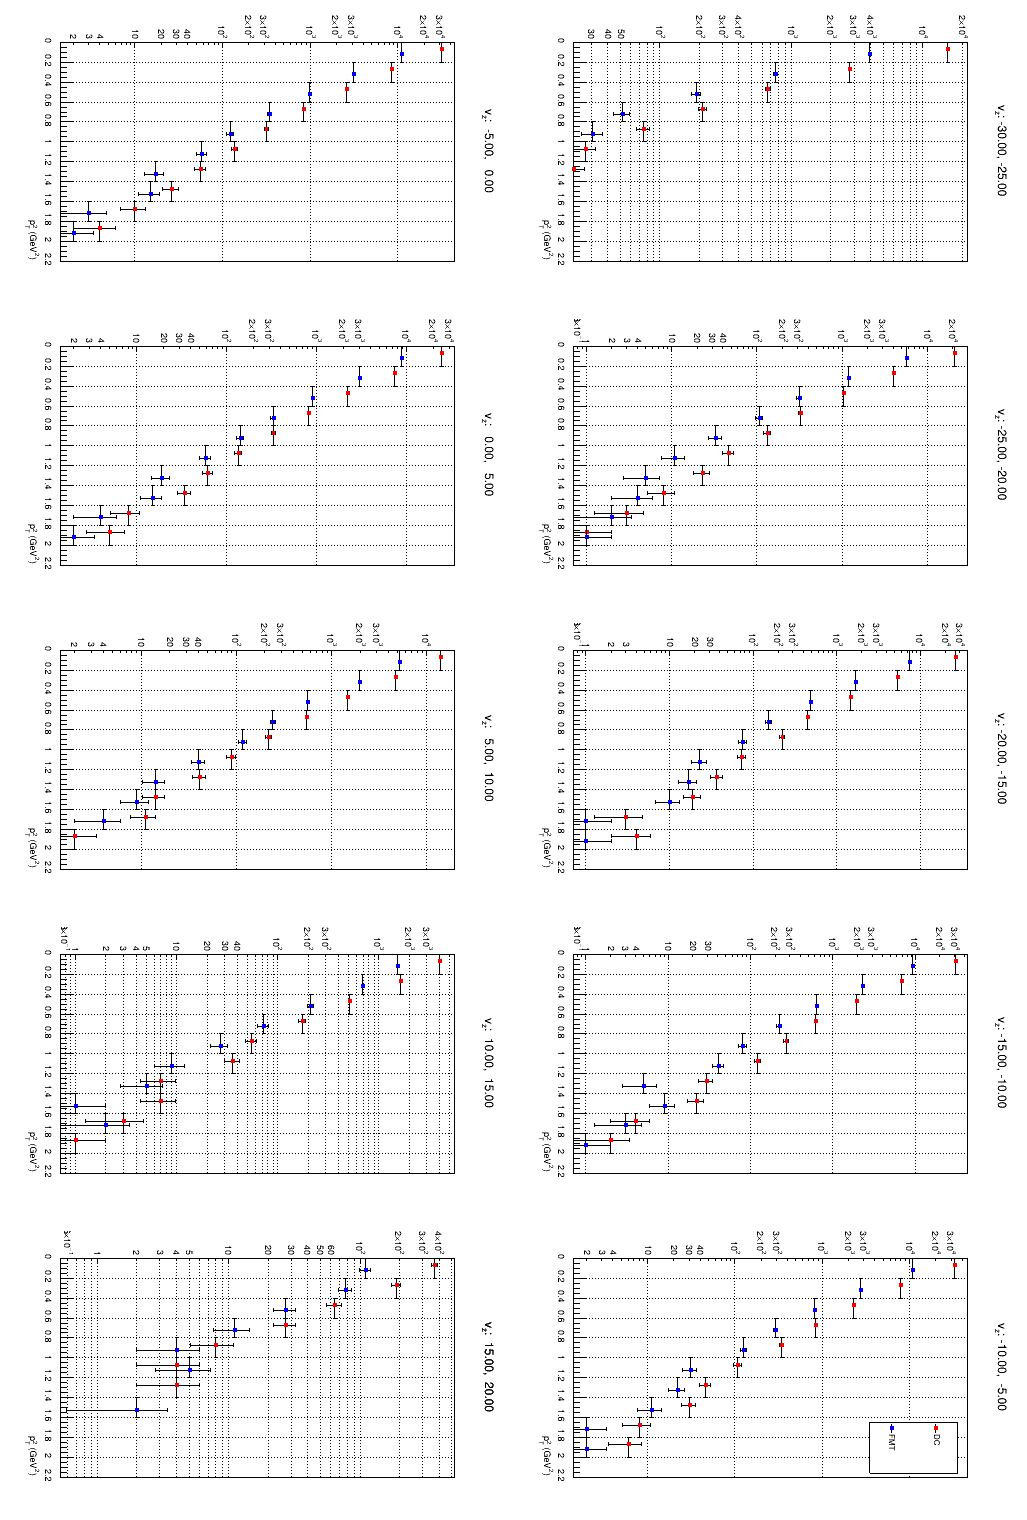
\includegraphics[width=\textwidth]{04pt2_vz_211.png}
        \caption[$p_T^2$ for $e^-\pi^+$ separated in $v_z$ bins]
        {$p_T^2$ for $e^-\pi^+$ detected by DC and FMT, separated in $v_z$ bins.
        Run 12016.
        The bin markers are slightly shifted in $x$ to improve legibility.}
        \floatfoot{Source: Own elaboration, using the \href{https://github.com/bleaktwig/clas12-rge-analysis}{clas12-rge-analysis} software.}
        \label{fig::20.04::pt2_211_vz}
    \end{figure}

    \begin{figure}
        \centering
        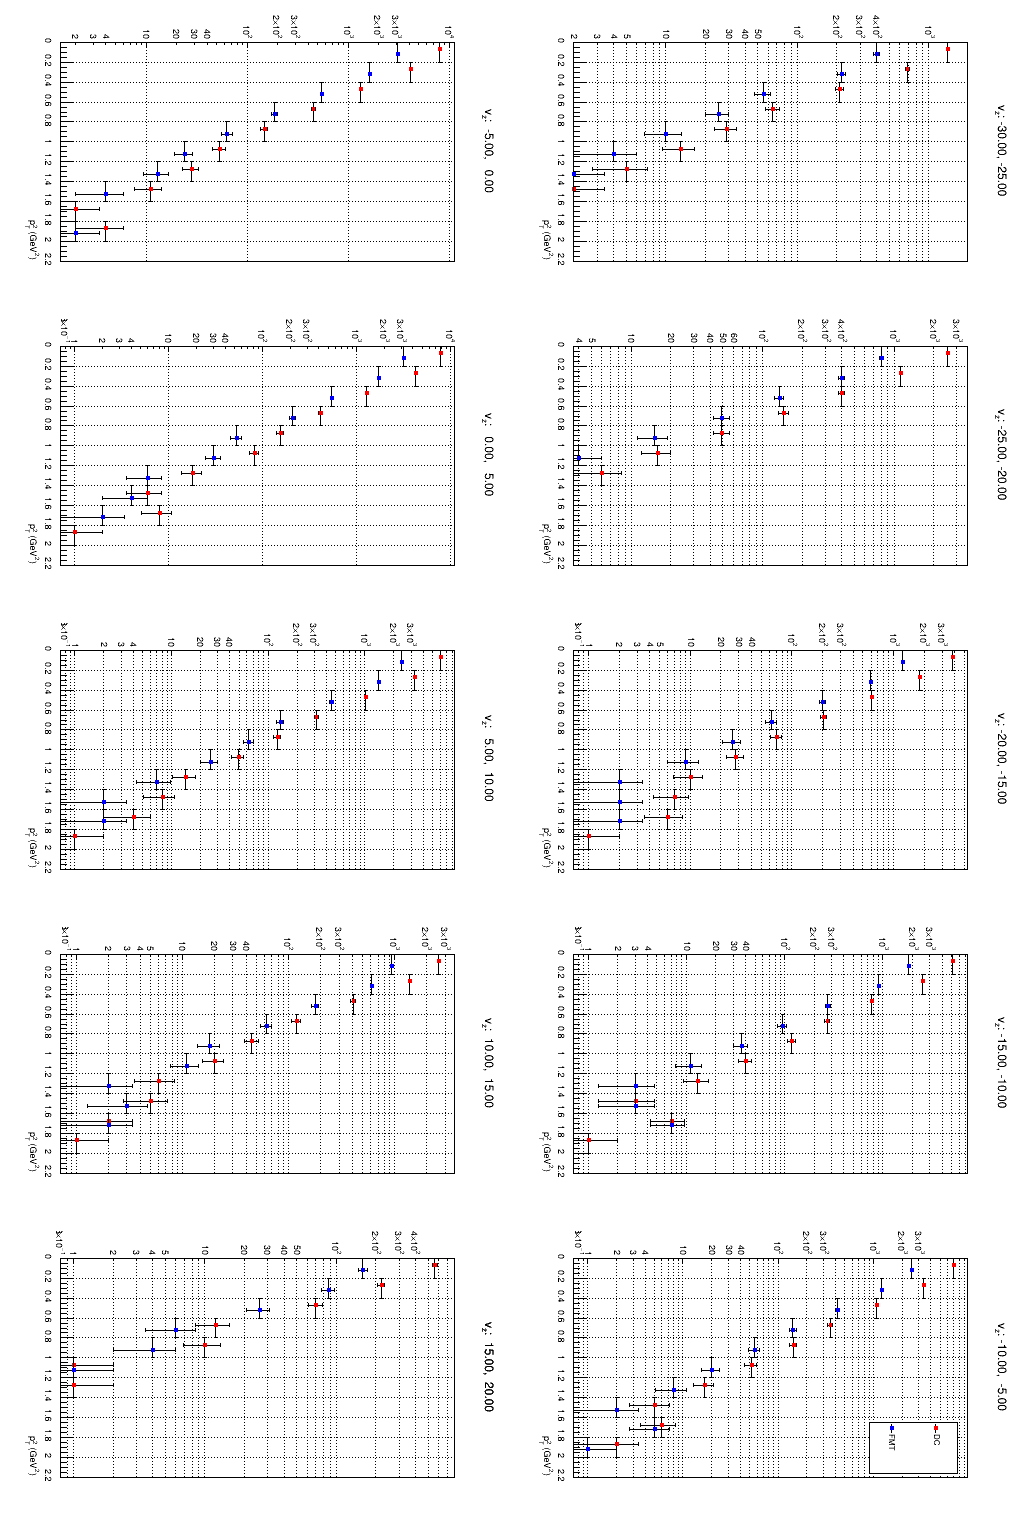
\includegraphics[width=\textwidth]{04pt2_vz_-211.png}
        \caption[$p_T^2$ for $e^-\pi^-$ separated in $v_z$ bins]
        {$p_T^2$ for $e^-\pi^-$ detected by DC and FMT, separated in $v_z$ bins.
        Run 12016.
        The bin markers are slightly shifted in $x$ to improve legibility.}
        \floatfoot{Source: Own elaboration, using the \href{https://github.com/bleaktwig/clas12-rge-analysis}{clas12-rge-analysis} software.}
        \label{fig::20.04::pt2_-211_vz}
    \end{figure}

    % phipq.
    \begin{figure}
        \centering
        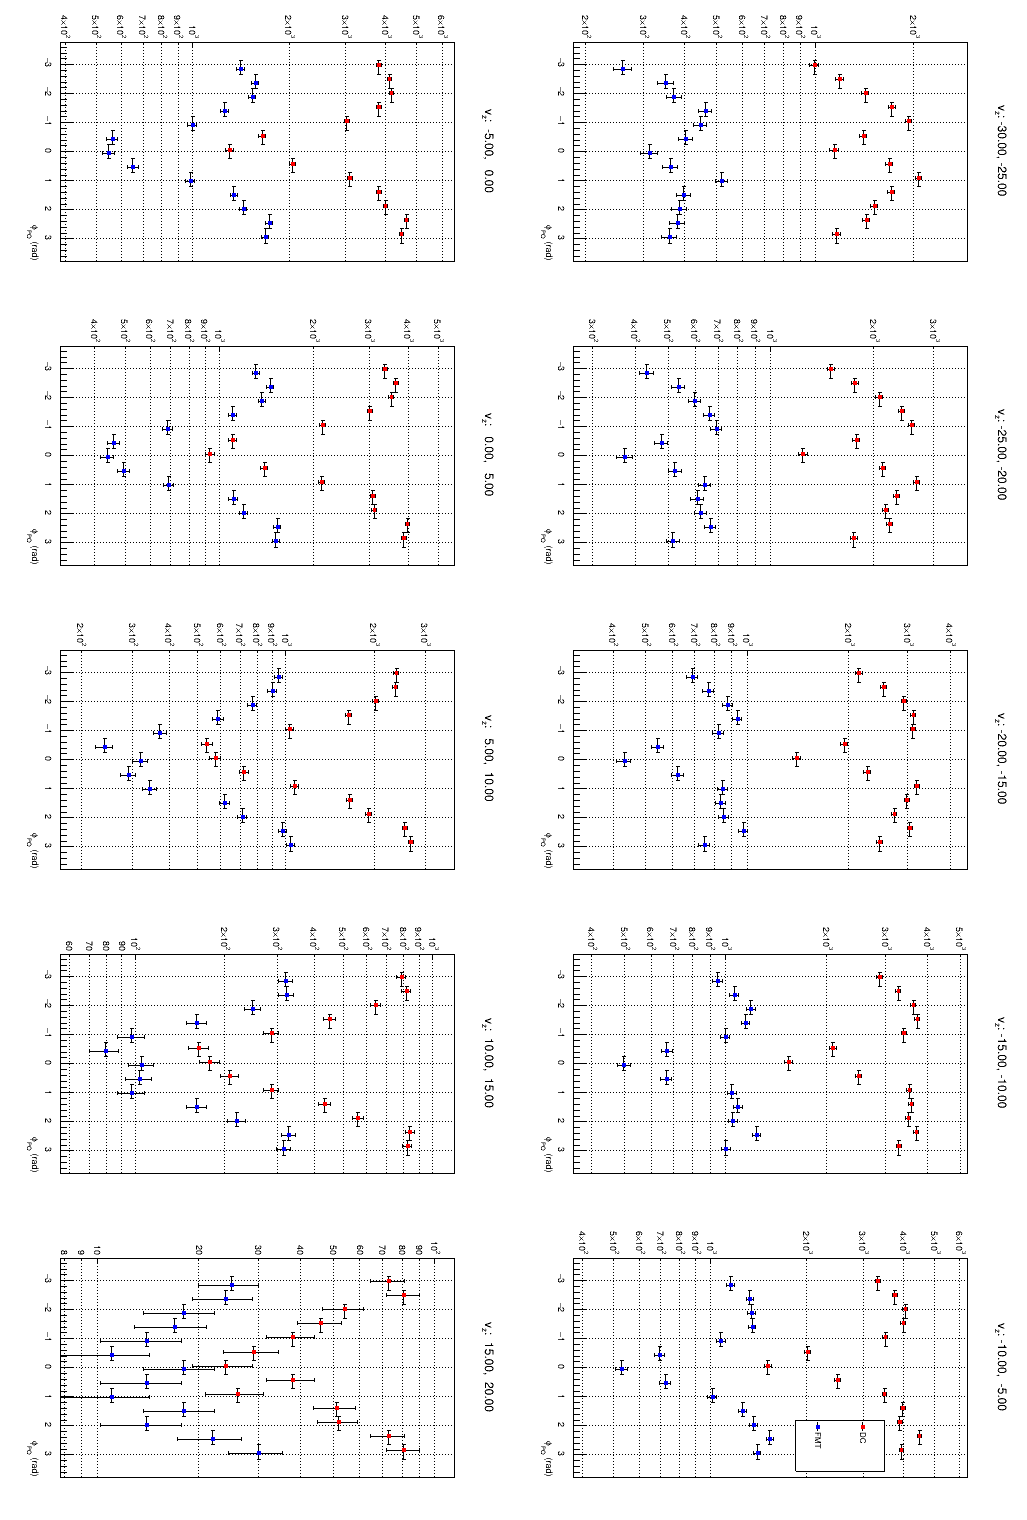
\includegraphics[width=\textwidth]{04phipq_vz_211.png}
        \caption[$\phi_{PQ}$ for $e^-\pi^+$ separated in $v_z$ bins]
        {$\phi_{PQ}$ for $e^-\pi^+$ detected by DC and FMT, separated in $v_z$ bins.
        Run 12016.
        The bin markers are slightly shifted in $x$ to improve legibility.}
        \floatfoot{Source: Own elaboration, using the \href{https://github.com/bleaktwig/clas12-rge-analysis}{clas12-rge-analysis} software.}
        \label{fig::20.04::phipq_211_vz}
    \end{figure}

    \begin{figure}
        \centering
        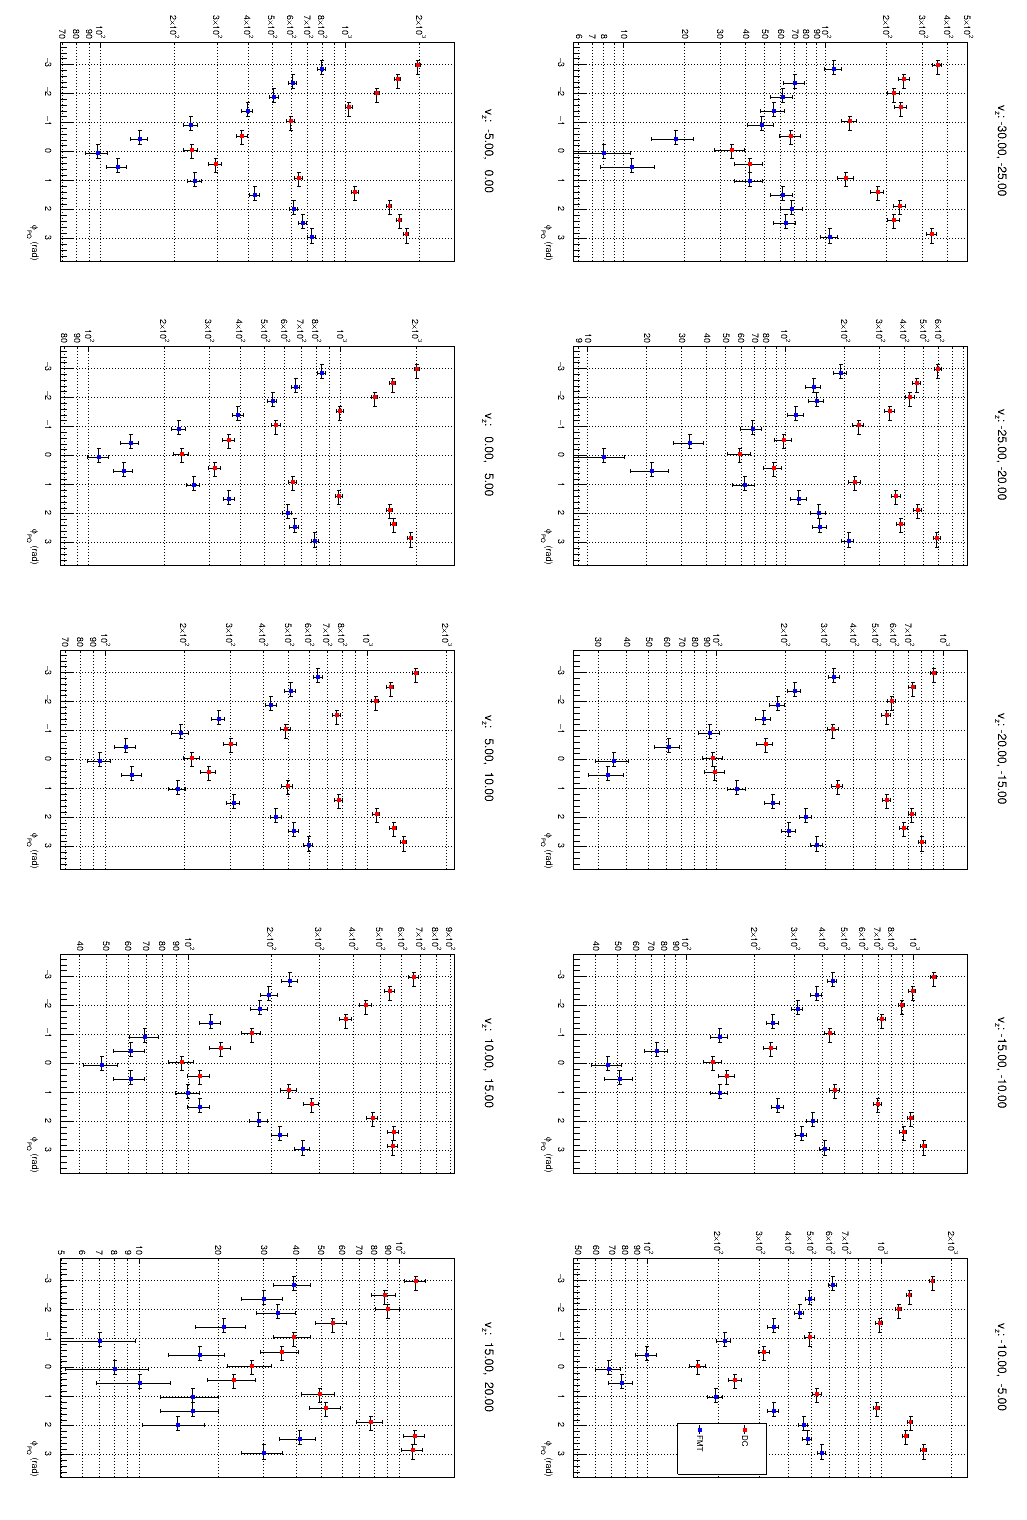
\includegraphics[width=\textwidth]{04phipq_vz_-211.png}
        \caption[$\phi_{PQ}$ for $e^-\pi^-$ separated in $v_z$ bins]
        {$\phi_{PQ}$ for $e^-\pi^-$ detected by DC and FMT, separated in $v_z$ bins.
        Run 12016.
        The bin markers are slightly shifted in $x$ to improve legibility.}
        \floatfoot{Source: Own elaboration, using the \href{https://github.com/bleaktwig/clas12-rge-analysis}{clas12-rge-analysis} software.}
        \label{fig::20.04::phipq_-211_vz}
    \end{figure}

    % \pagebreak

    % !TEX root = ../main.tex
\subsection{Fiducial Cuts}
\label{20.05::fiducial_cuts}
    % What are fiducial cuts?
    In detector physics, the fiducial region is defined as the region considered reliable and suitable for analysis.
    Fiducial cuts are constraints applied to experimental data in order to define this region.
    Thus, they allow us to exclude events or measurements that may be affected by experimental artefacts, detector inefficiencies, or other factors that could introduce systematic errors and biases \cite{leo1987}.

    % Why weren't fiducial cuts used in this thesis?
    Due to its 6-sector geometry, fiducial cuts are of particular importance for CLAS12 FD analysis.
    However, they were disregarded for this particular study.
    This is because of its broadness: we are only concerned with the phase space of DIS variables and the general statistics, as detailed in Section \ref{14.30::study_results}.
    While the cuts would likely improve the quality of the results, the data is broad enough to be considered resilient to the damage of not applying them.

    % How would we implement them?
    To apply such cuts, we would need to follow the procedure described in \cite{zana2010}.
    This would involve providing $\phi$ vs $\theta$ curves that cut all events at the edges of each DC sector.
    One curve would be needed for each $p$ bin, for each sector.
    Finally, different curves would be needed for each PID being processed.

    % Show plots.
    Examples of $\phi$ vs $\theta$ distributions for different $p$ bins can be seen in Figures \ref{fig::20.05::fiducial_cuts_pid11} and \ref{fig::20.05::fiducial_cuts_pid211}, where we show the distributions for $e^-$ and $\pi^+$.
    As can be seen in the plots, the separation between the detector sensitive area and its edges is easily observed.

    % e-.
    \begin{figure}
        \centering
        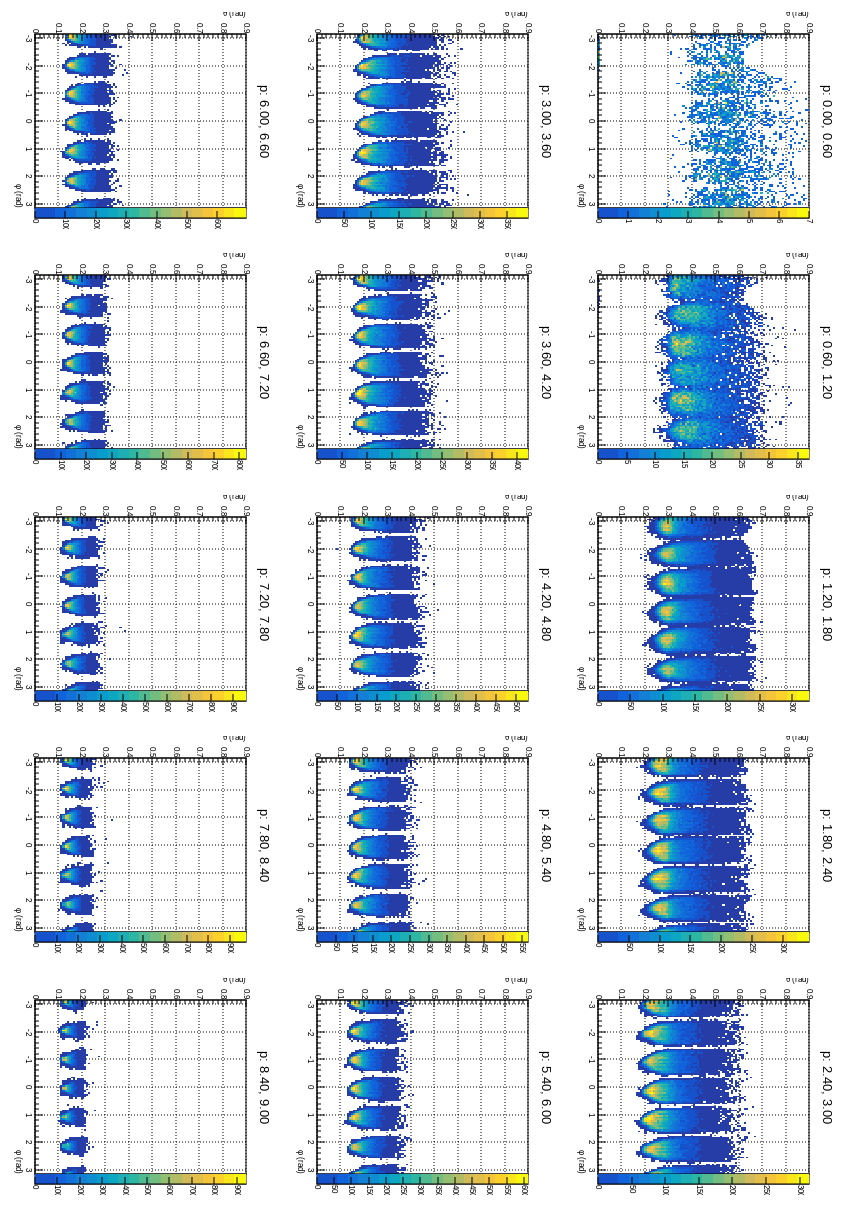
\includegraphics[width=\textwidth]{05fidcuts_11.png}
        \caption[$\phi$ vs $\theta$ of $e^-$ in $p$ bins]
        {$\phi$ vs $\theta$ of $e^-$ detected by DC, separated in $p$ bins.
        Run 12016.}
        \floatfoot{Source: Own elaboration, using the \href{https://github.com/bleaktwig/clas12-rge-analysis}{clas12-rge-analysis} software.}
        \label{fig::20.05::fiducial_cuts_pid11}
    \end{figure}

    % pi+.
    \begin{figure}
        \centering
        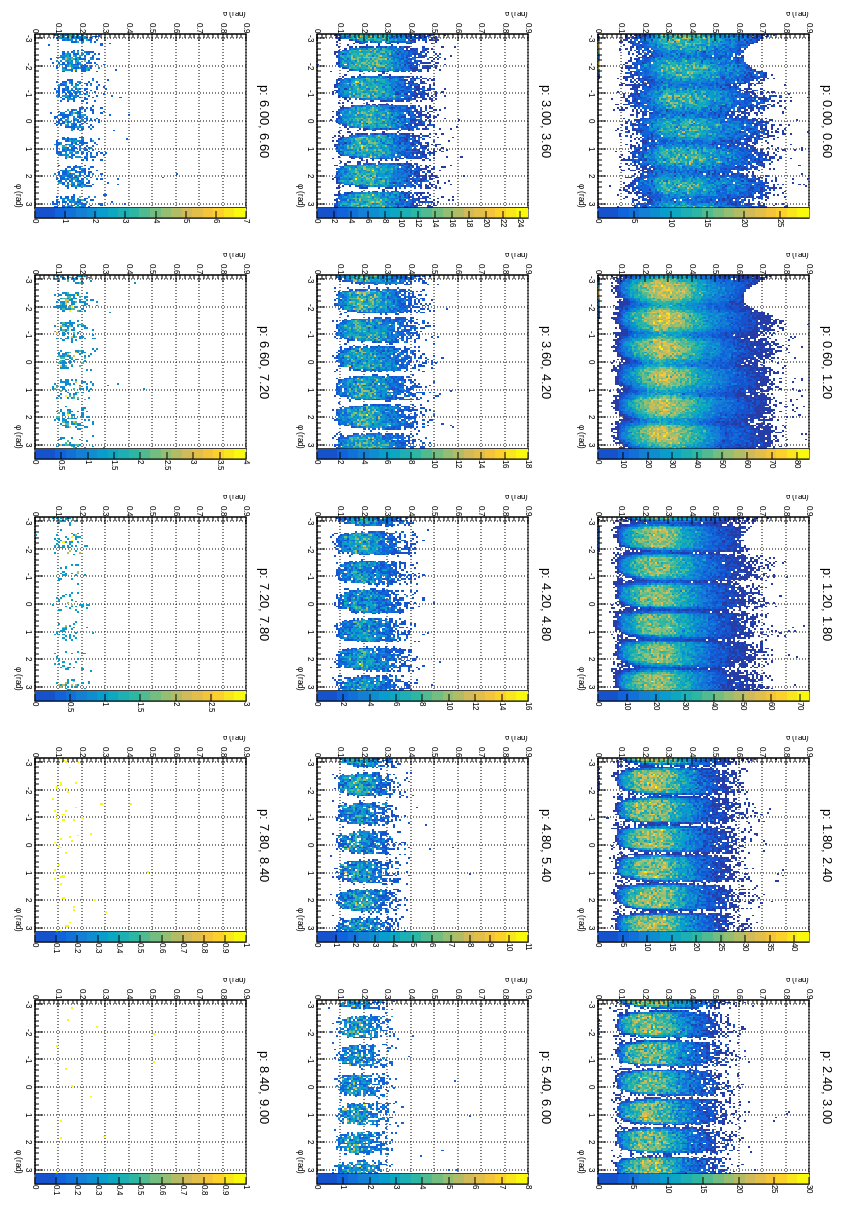
\includegraphics[width=\textwidth]{05fidcuts_211.png}
        \caption[$\phi$ vs $\theta$ of $\pi^+$ in $p$ bins]
        {$\phi$ vs $\theta$ of $\pi^+$ detected by DC, separated in $p$ bins.
        Run 12016.}
        \floatfoot{Source: Own elaboration, using the \href{https://github.com/bleaktwig/clas12-rge-analysis}{clas12-rge-analysis} software.}
        \label{fig::20.05::fiducial_cuts_pid211}
    \end{figure}



    % Run configuration.
    % All Figures in this section that show results for data are from RG-F run 12016.
    % For this run, a gas H2 target was used.
    % The beam energy was set to $10.4$ GeV, and the luminosity to $250$ nA.
    % The solenoid field was set to an inbending polarity ($-0.75$), and the torus to its regular polarity of $-1$.
    % The run has a total of $10,046,225$ events.
\end{document}
